\documentclass{beamer}
\usepackage[utf8]{inputenc}

\usetheme{Madrid}
\usecolortheme{default}
\usepackage{amsmath,amssymb,amsfonts,amsthm}
\usepackage{mathtools}
\usepackage{txfonts}
\usepackage{tkz-euclide}
\usepackage{listings}
\usepackage{adjustbox}
\usepackage{array}
\usepackage{gensymb}
\usepackage{tabularx}
\usepackage{gvv}
\usepackage{lmodern}
\usepackage{circuitikz}
\usepackage{tikz}
\lstset{literate={·}{{$\cdot$}}1 {λ}{{$\lambda$}}1 {→}{{$\to$}}1}
\usepackage{graphicx}

\setbeamertemplate{page number in head/foot}[totalframenumber]

\usepackage{tcolorbox}
\tcbuselibrary{minted,breakable,xparse,skins}



\definecolor{bg}{gray}{0.95}
\DeclareTCBListing{mintedbox}{O{}m!O{}}{%
  breakable=true,
  listing engine=minted,
  listing only,
  minted language=#2,
  minted style=default,
  minted options={%
    linenos,
    gobble=0,
    breaklines=true,
    breakafter=,,
    fontsize=\small,
    numbersep=8pt,
    #1},
  boxsep=0pt,
  left skip=0pt,
  right skip=0pt,
  left=25pt,
  right=0pt,
  top=3pt,
  bottom=3pt,
  arc=5pt,
  leftrule=0pt,
  rightrule=0pt,
  bottomrule=2pt,
  toprule=2pt,
  colback=bg,
  colframe=orange!70,
  enhanced,
  overlay={%
    \begin{tcbclipinterior}
    \fill[orange!20!white] (frame.south west) rectangle ([xshift=20pt]frame.north west);
    \end{tcbclipinterior}},
  #3,
}
\lstset{
    language=C,
    basicstyle=\ttfamily\small,
    keywordstyle=\color{blue},
    stringstyle=\color{orange},
    commentstyle=\color{green!60!black},
    numbers=left,
    numberstyle=\tiny\color{gray},
    breaklines=true,
    showstringspaces=false,
}
%------------------------------------------------------------
%This block of code defines the information to appear in the
%Title page
\title %optional
{9.4.39}
\date{September 10,2025}
%\subtitle{A short story}

\author % (optional)
{Harsha-EE25BTECH11026}



\begin{document}


\frame{\titlepage}


\begin{frame}{Question}
The difference of squares of two numbers is 180. The square of the smaller number is 8 times the larger number. Find the two numbers.
\end{frame}

\begin{frame}{Theoretical Solution}
Let x and y be the 2 numbers such that $x>y$.\\
The given equations are,
\begin{align}
    x^2-y^2=180 \label{eq:1}
\end{align}
\begin{align}
    y^2=8x \label{eq:2}
\end{align}
As the given equations are homogeneous, converting them into quadratic form,
\begin{align}
    \implies \vec{x}^{\top}\vec{V_1}\vec{x}+c=0 \label{eq:3}
\end{align}
where $\vec{x}^{\top}=\myvec{x&&y}$ and $\vec{V_1}=\myvec{1&&0\\0&&-1}$ and $c=-180$
\end{frame}

\begin{frame}{Theoretical Solution}
And also,
\begin{align}
    \vec{x}^{\top}\vec{V_2}\vec{x}+2\vec{u}^{\top}\vec{x}=0 \label{eq:4}
\end{align}
where $\vec{x}^{\top}=\myvec{x&&y}^{\top}$, $\vec{V_2}=\myvec{0&&0\\0&&1}$ and $\vec{u}=\myvec{-4\\0}$.\\
To identify the intersection of conics, we can employ the approach of degenerating the conics.\\
\\
To work with degeneracy in matrix form we form the standard augmented $3 \times 3$ matrix for each conic:
\begin{align}
    \vec{M_i}=\myvec{\vec{V_i}&&\vec{u_i}\\\vec{u_i}^{\top}&&c_i} \label{eq:5}
\end{align}
\end{frame}

\begin{frame}{Theoretical Solution}
From ~\eqref{eq:5},
\begin{align}
    \implies \vec{M_1}=\myvec{1&&0&&0\\0&&-1&&0\\0&&0&&-180} \quad 
    \vec{M_2}=\myvec{0&&0&&-4\\0&&1&&0\\-4&&0&&0}
\end{align}
\begin{align}
    \therefore \vec{x}^{\top}\brak{\vec{M_1+\lambda M_2}}\vec{x}=0
\end{align}
To degenerate the conic into a line, we can find the solutions of $\lambda$ when $\|\vec{M_1}+\lambda\vec{M_2}\|=0$ 
\begin{align}
    \therefore \|\vec{M_1}+\lambda\vec{M_2}\|=0 \label{eq:6}
\end{align}
\begin{align}
    \implies \brak{\lambda-1}\brak{4\lambda^2+45}=0
\end{align}
\begin{align}
    \therefore \lambda=1
\end{align}
\end{frame}

\begin{frame}{Theoretical Solution}
Substituting $\lambda$ in ~\eqref{eq:6},
\begin{align}
    \implies \vec{x}^{\top}\brak{\vec{M_1}+\vec{M_2}}\vec{x}
\end{align}
\begin{align}
    \implies x^2-8x-180=0
\end{align}
\begin{align}
    \implies x=18,-10
\end{align}
for $x=-10$, there is no real solution of $y$ in ~\eqref{eq:2},
\begin{align}
    \implies y=\pm 12
\end{align}
\begin{align}
    \therefore \text{The two numbers are }\brak{18,12}\, and\, \brak{18,-12}
\end{align}

\end{frame}

\begin{frame}[fragile]
    \frametitle{C Code -Finding the intersection of conics}

    \begin{lstlisting}[language=C]
#include <stdio.h>
#include <math.h>

void solve_conics(double *results) {
    // Quadratic in x: x^2 - 8x - 180 = 0
    double a = 1, b = -8, c = -180;
    double disc = b*b - 4*a*c;

    if (disc < 0) {
        // No real solution
        results[0] = results[1] = results[2] = results[3] = NAN;
        return;
    }

    // Roots of quadratic
    double sqrt_disc = sqrt(disc);
    double x1 = (-b + sqrt_disc) / (2*a);
    double x2 = (-b - sqrt_disc) / (2*a);


    \end{lstlisting}
\end{frame}

\begin{frame}[fragile]
    \frametitle{C Code -Finding the intersection of conics}

    \begin{lstlisting}[language=C]
    // Solutions
    int idx = 0;
    double xs[2] = {x1, x2};
    for (int i=0; i<2; i++) {
        double x = xs[i];
        if (x < 0) continue; // y^2 = 8x requires x >= 0
        double y2 = 8*x;
        double y = sqrt(y2);
        results[idx++] = x;
        results[idx++] = y;
        results[idx++] = x;
        results[idx++] = -y;
    }

    while (idx < 4) {
        results[idx++] = NAN;
    }
}
    \end{lstlisting}
\end{frame}




\begin{frame}[fragile]
    \frametitle{Python+C code}

    \begin{lstlisting}[language=Python]
import ctypes
import numpy as np
import matplotlib.pyplot as plt

# Load C shared library
lib = ctypes.CDLL("./libconics.so")

# Define return type
lib.solve_conics.argtypes = [ctypes.POINTER(ctypes.c_double)]

# Prepare results array
results = (ctypes.c_double * 4)()
lib.solve_conics(results)

vals = list(results)
points = [(vals[i], vals[i+1]) for i in range(0, len(vals), 2) if not np.isnan(vals[i])]
print("Solutions :", points)

    \end{lstlisting}
\end{frame}

\begin{frame}[fragile]
    \frametitle{Python+C code}

    \begin{lstlisting}[language=Python]
#   PLOT
fig, ax = plt.subplots(figsize=(6,6))
ax.set_xlabel("x")
ax.set_ylabel("y")
ax.set_title("Intersection of Hyperbola and Parabola")
ax.grid(True)

# Hyperbola: x^2 - y^2 = 180 -> y = ±sqrt(x^2 - 180)
xh = np.linspace(-40, 40, 800)
for sign in [1, -1]:
    yh = sign*np.sqrt(np.maximum(xh**2 - 180, 0))
    ax.plot(xh, yh, 'r', label="Hyperbola" if sign==1 else "")

# Parabola: y^2 = 8x -> y = ±sqrt(8x)
xp = np.linspace(0, 40, 400)
for sign in [1, -1]:
    yp = sign*np.sqrt(8*xp)
    ax.plot(xp, yp, 'b', label="Parabola" if sign==1 else "")

    \end{lstlisting}
\end{frame}

\begin{frame}[fragile]
    \frametitle{Python+C code}

    \begin{lstlisting}[language=Python]
   
# Intersection points from C
for (px, py) in points:
    ax.plot(px, py, 'ko', markersize=8)
    ax.text(px+0.5, py+0.5, f"({px:.0f},{py:.0f})")

ax.legend()
plt.savefig("/home/user/Matrix Theory: workspace/Matgeo_assignments/9.4.39/figs/Figure_1.png")
plt.show()

    \end{lstlisting}
\end{frame}

\begin{frame}[fragile]
    \frametitle{Python code}
    \begin{lstlisting}[language=Python]
import sympy as sp
import numpy as np
import matplotlib.pyplot as plt

# Variables
x, y = sp.symbols('x y', real=True)
# Equations
eq1 = sp.Eq(x**2 - y**2, 180)   # Hyperbola
eq2 = sp.Eq(y**2, 8*x)          # Parabola
# Solve system
solutions = sp.solve([eq1, eq2], [x, y], dict=True)
print("Solutions:")
for sol in solutions:
    print(sol)
# Extract real solutions
real_solutions = [(float(sol[x]), float(sol[y])) for sol in solutions if sol[y].is_real]
    \end{lstlisting}   
\end{frame}

\begin{frame}[fragile]
    \frametitle{Python code}
    \begin{lstlisting}[language=Python]
# Setup plot
fig, ax = plt.subplots(figsize=(6,6))
ax.set_xlabel("x")
ax.set_ylabel("y")
ax.set_title("Intersection of Hyperbola and Parabola")
ax.grid(True)

# Range for plotting
xx = np.linspace(-20, 40, 400)

# Hyperbola: x^2 - y^2 = 180 -> y = ±sqrt(x^2 - 180)
xh = np.linspace(-40, 40, 800)
for sign in [1, -1]:
    yh = sign*np.sqrt(np.maximum(xh**2 - 180, 0))  # avoid negatives under sqrt
    ax.plot(xh, yh, 'r', label="Hyperbola" if sign==1 else "")
    \end{lstlisting}   
\end{frame}

\begin{frame}[fragile]
    \frametitle{Python code}
    \begin{lstlisting}[language=Python]
# Parabola: y^2 = 8x -> y = ±sqrt(8x)
xp = np.linspace(0, 40, 400)  # parabola domain x>=0
for sign in [1, -1]:
    yp = sign*np.sqrt(8*xp)
    ax.plot(xp, yp, 'b', label="Parabola" if sign==1 else "")
# Mark intersection points
for (px, py) in real_solutions:
    ax.plot(px, py, 'ko', markersize=8)
    ax.text(px+0.5, py+0.5, f"({px:.0f},{py:.0f})")

ax.legend()
plt.savefig("/home/user/Matrix Theory: workspace/Matgeo_assignments/9.4.39/figs/Figure_1.png")
plt.show()
    \end{lstlisting}   
\end{frame}

\begin{frame}{Plot}
    \begin{figure}[H]
    \centering
    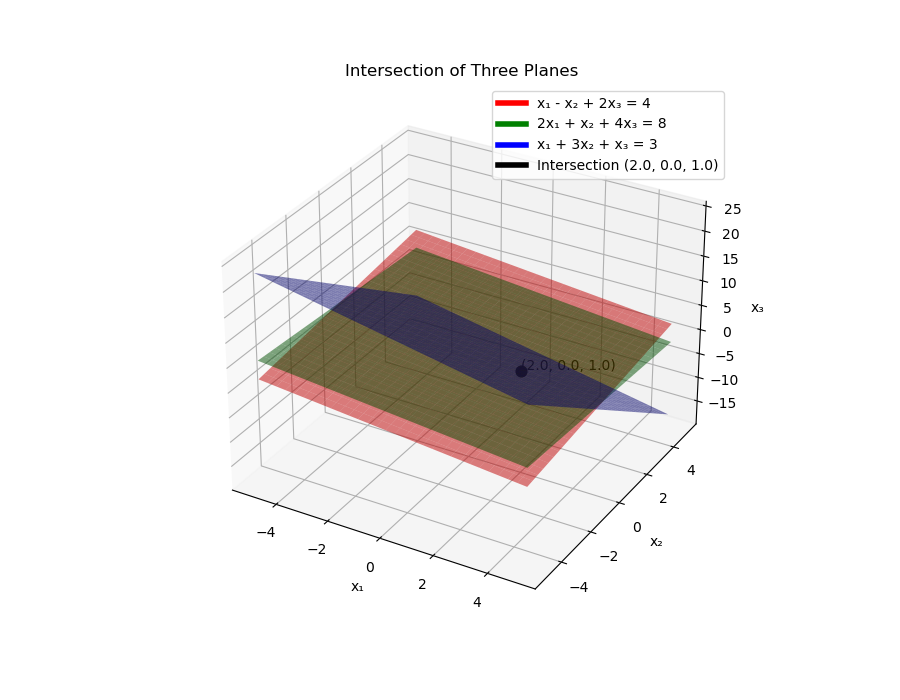
\includegraphics[width=0.6\columnwidth]{figs/Figure_1.png}
    \label{fig:1}
\end{figure}
\end{frame}

\end{document}
